\documentclass[11pt]{article} 
% ~~~~~~~~~~~~~~~~~~~~~~~~~~~~~~~~~~~~~~~~~~~~~~~~~~~~~ %
\usepackage{etex}													%
\usepackage[english]{babel}											%
\usepackage[a4paper,margin=3cm]{geometry}							%
\usepackage{dsfont}													%
\usepackage{booktabs}												%
\usepackage{array}													%
\usepackage{bm}														%
\usepackage{enumerate}												%
\usepackage[table]{xcolor}											%
\usepackage{amsmath,amssymb,amsfonts}								% 
\usepackage{multirow}												%
\usepackage{graphicx}												% 
\DeclareGraphicsExtensions{.pdf,.png,.jpg,.mps}						%
\usepackage[colorlinks=true,linkcolor=black!90!white]{hyperref}		%
\usepackage{framed}													%
\usepackage[amsmath,thmmarks,framed,hyperref]{ntheorem}				%
\usepackage{pdftexcmds}												%
\usepackage{eso-pic}												%
\usepackage[switch, pagewise, mathlines]{lineno}					%
\usepackage[color=red!20!white, textwidth=5cm]{todonotes}			%
\usepackage{algorithm}												%
\usepackage[noend]{algpseudocode}									%
\usepackage{acronym}												%
\usepackage{subcaption}												%
\usepackage{url}													%
\usepackage{bm}														%
\usepackage{tikz}				% (note: AFTER \pdfminorversion)	%
\usepackage{pgfplots}												%
\let\labelindent\relax												%
\usepackage{enumitem}												%
\everymath={\displaystyle}											%
\usepackage{mathtools}												%
\usepackage{textcomp}												%
\usetikzlibrary{shapes,arrows}										%
% ~~~~~~~~~~~~~~~~~~~~~~~~~~~~~~~~~~~~~~~~~~~~~~~~~~~~~~~~~~~~~~~~~ %

	
% --> numbered environments style ridefinition example:
%
%\newtheoremstyle{mystyle}	% name of the style
%{3pt}						% vertical space before the environment
%{8pt}						% vertical space after the environment
%{}							% body's font
%{}							% indentation (empty -> \parindent)
%{\bfseries}				% header's font
%{.}						% punctuation after the header
%{\newline}					% space after the header (empty -> \newline)
%{\thmname{#1}\thmnumber{ #2}\thmnote{ #3}}	% header formatting
%											% (cancel for the default)
%
%
% --> numbered environments ridefinition example
%
% \newtheorem	{unique_name}			% environment's ID
%										% (use \begin{unique_name})
%				[associated_counter]	% [optional] could be not
%										% unambiguous
%				{text}					% what will be printed
%				[section]				% [optional] to which kind of
%										% sectioning the enumeration
%										% will be tied



\theoremstyle		{nonumberplain}
\def\theoremframecommand{\colorbox[rgb]{0.95,0.95,0.95}}
\newshadedtheorem	{instructions}		{Instructions:}


% in order to call \includegraphics{myImage} instead of \includegraphics{../images/myImage}
\graphicspath{{../Images/}}

\pgfdeclarelayer{ultrabackground}
\pgfdeclarelayer{background}
\pgfdeclarelayer{foreground}
\pgfsetlayers{ultrabackground,background,main,foreground}


% \begin{pgfonlayer}{foreground}
% 	%
% 	%
% \end{pgfonlayer}


\def\TablesRowsColor{black!8}
\def\TablesColumnsColor{black!4}

\newcolumntype
{g}
{
	>{\centering \columncolor{\TablesColumnsColor} \arraybackslash}
	p{0.15\textwidth}
	<{}
}

\newcolumntype
{w}
{
	>{\centering \arraybackslash}
	p{0.15\textwidth}
	<{}
}


\newcommand{\source}[1]
{
	\ifthenelse
	{\boolean{writefilenames}}
	{
		\begin{center}
		{\color[rgb]{0.6,0.6,0.6} \rule{\columnwidth}{0.2mm}}
		$\downarrow\;\;$ \textbf{#1} $\;\;\downarrow$
		\end{center}
	}
	{}
}


\newcommand{\EstimatedSignal}						[0]	{\widehat{\Signal}}
\newcommand{\OptimallyEstimatedSignal}				[0]	{\widehat{\Signal}^{*}}
\newcommand{\OptimallyBayesEstimatedSignal}			[0]	{\widehat{\Signal}^{*}_{\text{Bayes}}}
\newcommand{\OptimallyCostFunctionEstimatedSignal}	[0]	{\widehat{\Signal}^{*}_{\text{c.f.}}}
%
\newcommand{\EstimatedSignalAt}						[1]	{\EstimatedSignal \left( #1 \right)}
\newcommand{\OptimallyEstimatedSignalAt}			[1]	{\OptimallyEstimatedSignal \left( #1 \right)}
\newcommand{\OptimallyBayesEstimatedSignalAt}		[1]	{\OptimallyBayesEstimatedSignal \left( #1 \right)}
\newcommand{\OptimallyCostFunctionEstimatedSignalAt}[1]	{\OptimallyCostFunctionEstimatedSignal \left( #1 \right)}
%
\newcommand{\EstimatedSignalAtSet}						[1]	{\EstimatedSignal_{#1}}
\newcommand{\OptimallyEstimatedSignalAtSet}				[1]	{\OptimallyEstimatedSignal_{#1}}
\newcommand{\OptimallyBayesEstimatedSignalAtSet}		[1]	{\OptimallyBayesEstimatedSignal_{#1}}
\newcommand{\OptimallyCostFunctionEstimatedSignalAtSet}	[1]	{\OptimallyCostFunctionEstimatedSignal_{#1}}




\newcommand{\EstimatedEigenfunctionWeight}			[1]
			{\widehat{a}_{#1}}
\newcommand{\SetOfEstimatedEigenfunctionsWeights}	[0]
			{\widehat{\SetOfEigenfunctionsWeights}}
\newcommand{\EigenfunctionsWeightsEstimationError}	[0]
			{\widetilde{\SetOfEigenfunctionsWeights}}




\newcommand{\EstimatedEigenfunctionWeightOfSensor}			[2]
			{\widehat{a}_{#1, #2}}
\newcommand{\SetOfEstimatedEigenfunctionsWeightsOfSensor}	[1]
			{\widehat{\SetOfEigenfunctionsWeights}_{#1}}
\newcommand{\EigenfunctionsWeightsEstimationErrorOfSensor}	[1]
			{\widetilde{\SetOfEigenfunctionsWeights}_{#1}}
\newcommand{\LocallyEstimatedEigenfunctionWeightOfSensor}	[2]
			{\widehat{a}_{#1, #2}^{loc}}




\newcommand{\SetOfLocallyEstimatedEigenfunctionsWeights}				[0]
			{\widehat{\SetOfEigenfunctionsWeights}^{\text{loc}}}
\newcommand{\SetOfLocallyEstimatedEigenfunctionsWeightsOfSensor}		[1]
			{\widehat{\SetOfEigenfunctionsWeights}^{\text{loc}}_{#1}}
\newcommand{\SetOfLocallyBayesEstimatedEigenfunctionsWeights}			[0]
			{\widehat{\SetOfEigenfunctionsWeights}_{\text{Bayes}}^{\text{loc}}}
\newcommand{\SetOfLocallyCostFunctionEstimatedEigenfunctionsWeights}	[0]
			{\widehat{\SetOfEigenfunctionsWeights}_{\text{c.f.}}^{\text{loc}}}
%
\newcommand{\SetOfLocallyBayesEstimatedEigenfunctionsWeightsOfSensor}			[1]
			{\widehat{\SetOfEigenfunctionsWeights}_{\text{Bayes}, #1}^{\text{loc}}}
\newcommand{\SetOfLocallyCostFunctionEstimatedEigenfunctionsWeightsOfSensor}	[1]
			{\widehat{\SetOfEigenfunctionsWeights}_{\text{c.f.}, #1}^{\text{loc}}}
%
%
\newcommand{\SetOfCentrallyEstimatedEigenfunctionsWeights}				[0]
			{\widehat{\SetOfEigenfunctionsWeights}^{\text{cen}}}
\newcommand{\SetOfCentrallyBayesEstimatedEigenfunctionsWeights}			[0]
			{\widehat{\SetOfEigenfunctionsWeights}_{\text{Bayes}}^{\text{cen}}}
\newcommand{\SetOfCentrallyCostFunctionEstimatedEigenfunctionsWeights}	[0]
			{\widehat{\SetOfEigenfunctionsWeights}_{\text{c.f.}}^{\text{cen}}}
%
\newcommand{\SetOfCentrallyBayesEstimatedEigenfunctionsWeightsOfSensor}			[1]
			{\widehat{\SetOfEigenfunctionsWeights}_{\text{Bayes}, #1}^{\text{cen}}}
\newcommand{\SetOfCentrallyCostFunctionEstimatedEigenfunctionsWeightsOfSensor}	[1]
			{\widehat{\SetOfEigenfunctionsWeights}_{\text{c.f.}, #1}^{\text{cen}}}
%
%
\newcommand{\SetOfDistributelyEstimatedEigenfunctionsWeights}				[0]
			{\widehat{\SetOfEigenfunctionsWeights}^{\text{dis}}}
\newcommand{\SetOfDistributelyBayesEstimatedEigenfunctionsWeights}			[0]
			{\widehat{\SetOfEigenfunctionsWeights}_{\text{Bayes}}^{\text{dis}}}
\newcommand{\SetOfDistributelyCostFunctionEstimatedEigenfunctionsWeights}	[0]
			{\widehat{\SetOfEigenfunctionsWeights}_{\text{c.f.}}^{\text{dis}}}
%
\newcommand{\SetOfDistributelyBayesEstimatedEigenfunctionsWeightsOfSensor}			[1]
			{\widehat{\SetOfEigenfunctionsWeights}_{\text{Bayes}, #1}^{\text{dis}}}
\newcommand{\SetOfDistributelyCostFunctionEstimatedEigenfunctionsWeightsOfSensor}	[1]
			{\widehat{\SetOfEigenfunctionsWeights}_{\text{c.f.}, #1}^{\text{dis}}}




\newcommand{\MaxAdmittableDistanceBtwOptimalCentralizedAndSuboptimalDistributedEstimates}	[0]
			{d_{\text{o.c.}-\text{s.d.}}^{\text{max}}}



\newcommand{\DistanceBtwLocalApproximatedBayesAndLocalApproximatedCostFunction}	[0]
	{d_{\text{l.a.B. - l.a.c.f.}}}
\newcommand{\DistanceBtwLocalOptimalBayesAndLocalApproximatedCostFunction}		[0]
	{d_{\text{l.o.B. - l.a.c.f.}}}
\newcommand{\DistanceBtwLocalOptimalBayesAndLocalApproximatedBayes}				[0]
	{d_{\text{l.o.B. - l.a.B.}}}



\newcommand{\NaiveDistributedEstimatorOfEigenfunctionsWeights}		[0]
	{\widehat{\SetOfEigenfunctionsWeights}_{\text{dis}}^{\text{naive}}}
%
\newcommand{\GuessedDistributedEstimatorOfEigenfunctionsWeights}	[0]
	{\widehat{\SetOfEigenfunctionsWeights}_{\text{dis}}^{\text{guess}}}
\newcommand{\GuessedDistributedEstimatorOfEigenfunctionsWeightsOfGuess}	[1]
	{\GuessedDistributedEstimatorOfEigenfunctionsWeights \left( #1 \right)}




\newcommand{\DefinedAs}			[0]	{\mathrel{\mathop:}=}
\newcommand{\IDefinedAs}		[0]	{=\mathrel{\mathop:}}
%\newcommand{\DefinedAs}			[0]	{\mathrel{\doteq}}
%\newcommand{\IDefinedAs}		[0]	{\mathrel{\doteq}}


\newcommand{\ExponentialOf}		[1]	{\mathrm{exp} \left( #1 \right)}
\newcommand{\LogarithmOf}		[1]	{\mathrm{ln} \left( #1 \right)}
\newcommand{\ConvexHullOf}		[1]	{\mathcal{H}_{\textrm{cvx}} \left( #1 \right)}
\newcommand{\ConicalHullOf}		[1]	{\mathcal{H}_{\textrm{cnc}} \left( #1 \right)}
\newcommand{\BoundaryOf}		[1]	{\mathcal{B} \left( #1 \right)}
\newcommand{\InteriorOf}		[1]	{\mathrm{int} \left( #1 \right)}
\newcommand{\MeasureOfIn}		[2]	{\mu_{#2} \left( #1 \right)}


\newcommand{\MaximumOfOne}		[1]	{\mathrm{max} \left\lbrace #1 \right\rbrace}
\newcommand{\MaximumOfTwo}		[2]	{\mathrm{max} \left\lbrace #1, #2 \right\rbrace)}
\newcommand{\MaximumOfThree}	[3]	{\mathrm{max} \left\lbrace #1, #2, #3 \right\rbrace)}
\newcommand{\MinimumOfOne}		[1]	{\mathrm{min} \left\lbrace #1 \right\rbrace}
\newcommand{\MinimumOfTwo}		[2]	{\mathrm{min} \left\lbrace #1, #2 \right\rbrace)}
\newcommand{\MinimumOfThree}	[3]	{\mathrm{min} \left\lbrace #1, #2, #3 \right\rbrace)}


\newcommand{\CostFunction}				[0]	{Q}
\newcommand{\CostFunctionOf}			[1]	{\CostFunction \left( #1 \right)}
\newcommand{\CostFunctionOfSensor}		[1]	{\CostFunction_{#1}}
\newcommand{\CostFunctionOfSensorOf}	[2]	{\CostFunctionOfSensor{#1} \left( #2 \right)}


\newcommand{\KroneckerDeltaOf}			[2]	{\delta_{#1 #2}}


\newcommand{\FloorOf}			[1]	{\lfloor #1 \rfloor}
\newcommand{\CeilOf}			[1]	{\lceil #1 \rceil}
\newcommand{\SaturationOf}		[1]	{\mathrm{sat} \left( #1 \right)}
\newcommand{\PositivePartOf}	[1]	{\left[ #1 \right]_{+}}
\newcommand{\NegativePartOf}	[1]	{\left[ #1 \right]_{-}}


\newcommand{\GammaFunctionOf}	[1]	{\Gamma \left( #1 \right)}
\newcommand{\BetaFunctionOf}	[2]	{B \left( #1, #2 \right)}


\newcommand{\CholeskyFactorOf}	[1]	{\mathrm{chol} \left( #1 \right)}


\newcommand{\BigOOf}			[1]	{O \left( #1 \right)}
\newcommand{\SmallOOf}			[1]	{o \left( #1 \right)}


\newcommand{\PochhammerOf}		[2]	{\left( #1 \right)_{#2}}


\DeclareMathOperator*{\argmax}{arg\,max}
\DeclareMathOperator*{\argmin}{arg\,min}

\newcommand{\SensorIndex}			{s}
\newcommand{\SensorIndexTwo}		{r}
\newcommand{\SensorIndexThree}		{q}
%
\newcommand{\MeasurementIndex}		{m}
\newcommand{\MeasurementIndexTwo}	{n}
\newcommand{\MeasurementIndexThree}	{p}
%
\newcommand{\TimeIndex}				{t}
\newcommand{\TimeIndexTwo}			{\tau}
\newcommand{\TimeIndexThree}		{\tau'}
%
\newcommand{\EigenvalueIndex}		{k}
\newcommand{\EigenvalueIndexTwo}	{i}
\newcommand{\EigenvalueIndexThree}	{g}
%
\newcommand{\EigenvectorIndex}		{\EigenvalueIndex}
\newcommand{\EigenvectorIndexTwo}	{\EigenvalueIndexTwo}
\newcommand{\EigenvectorIndexThree}	{\EigenvalueIndexThree}
%
\newcommand{\EigenfunctionIndex}		{\EigenvalueIndex}
\newcommand{\EigenfunctionIndexTwo}		{\EigenvalueIndexTwo}
\newcommand{\EigenfunctionIndexThree}	{\EigenvalueIndexThree}



\newcommand{\NumberOfEigenvalues}					[0]	{E}
\newcommand{\NumberOfEigenvectors}					[0]	{\NumberOfEigenvalues}
\newcommand{\NumberOfEigenfunctions}				[0]	{\NumberOfEigenvalues}
\newcommand{\NumberOfSensors}						[0]	{S}
\newcommand{\NumberOfMeasurements}					[0]	{M}
\newcommand{\NumberOfMeasurementsOfSensor}			[1]	{\NumberOfMeasurements_{#1}}
\newcommand{\NumberOfMeasurementsOfAuxiliaryGrid}	[0]	{\NumberOfMeasurements_{G}}
\newcommand{\NumberOfInputLocations}				[0]	{\NumberOfMeasurements}
\newcommand{\NumberOfInputLocationsOfSensor}		[1]	{\NumberOfMeasurements_{#1}}
\newcommand{\NumberOfInputLocationsOfAuxiliaryGrid}	[0]	{\NumberOfMeasurements_{G}}
\newcommand{\NumberOfTimeIndexes}					[0]	{T}



\newcommand{\DimensionOfInputLocationsDomain}		[0]	{D}
\newcommand{\IdentityMatrix}		[1]	{I_{#1}}
\newcommand{\DiagonalMatrixOf}		[1]	{\mathrm{diag} \left( #1 \right)}
\newcommand{\OnesVector}			[0]	{\mathds{1}}

\newcommand{\TraceOf}				[1]	{\mathrm{tr} \left( #1 \right)}
\newcommand{\DeterminantOf}			[1]	{\mathrm{det} \left( #1 \right)}

\newcommand{\Eigenvalue}			[0]	{\lambda}
\newcommand{\EigenvalueOfIndex}		[1]	{\Eigenvalue_{#1}}
\newcommand{\MaximalEigenvalue}		[0]	{\Eigenvalue_{\mathrm{max}}}
\newcommand{\MinimalEigenvalue}		[0]	{\Eigenvalue_{\mathrm{min}}}
\newcommand{\SetOfEigenvaluesOf}	[1]	{\mathrm{eig} \left( #1 \right)}

\newcommand{\Eigenvector}			[0]	{v}
\newcommand{\EigenvectorOfIndex}	[1]	{\Eigenvector_{#1}}

\newcommand{\SpectralRadius}		[0]	{\mu}
\newcommand{\SpectralRadiusOf}		[1]	{\SpectralRadius \left( #1 \right)}

\newcommand{\KernelOf}				[1]	{\mathrm{Ker} \left( #1 \right)}
\newcommand{\SpanOf}				[1]	{\mathrm{span} \left\langle #1 \right\rangle}

\newcommand{\VectorizationOf}		[1] {\mathrm{vec} \left( #1 \right)}
\newcommand{\HalfVectorizationOf}	[1] {\mathrm{vech} \left( #1 \right)}
\newcommand{\MatricizationOf}		[1] {\mathrm{mat} \left( #1 \right)}
\newcommand{\HalfMatricizationOf}	[1] {\mathrm{math} \left( #1 \right)}


\newcommand{\GaussianDistribution}					[2]	{\mathcal{N} \left( #1, #2 \right)}
\newcommand{\GammaDistribution}						[2]	{\mathrm{Gamma} \left( #1, #2 \right)}
\newcommand{\InverseGammaDistribution}				[2]	{\mathrm{Inv-Gamma} \left( #1, #2 \right)}
\newcommand{\ChiSquareDistribution}					[0]	{\chi^{2}}
\newcommand{\ChiSquareDistributionOfIndex}			[1]	{\ChiSquareDistribution \left( #1 \right)}
\newcommand{\InverseChiSquareDistribution}			[0]	{\mathrm{Inv-}\chi^{2}}
\newcommand{\InverseChiSquareDistributionOfIndex}	[1]	{\InverseChiSquareDistribution \left( #1 \right)}
\newcommand{\UniformDistribution}					[2]	{\mathcal{U} \left[ #1, #2 \right]}
\newcommand{\ExponentialDistribution}				[1]	{\mathrm{Exp} \left( #1 \right)}
\newcommand{\BernoulliDistribution}					[1]	{\mathcal{B} \left( #1 \right)}
\newcommand{\BinomialDistribution}					[2]	{\mathrm{Bin} \left( #1, #2 \right)}


\newcommand{\SetOfComplexNumbers}					[0]	{\mathbb{C}}
\newcommand{\SetOfRealNumbers}						[0]	{\mathbb{R}}
\newcommand{\SetOfRealPositiveNumbers}				[0]	{\mathbb{R}_{+}}
\newcommand{\SetOfRationalNumbers}					[0]	{\mathbb{Q}}
\newcommand{\SetOfRationalPositiveNumbers}			[0]	{\mathbb{Q}_{+}}
\newcommand{\SetOfNaturalNumbers}					[0]	{\mathbb{N}}
\newcommand{\SetOfNaturalPositiveNumbers}			[0]	{\mathbb{N}_{+}}

\newcommand{\SetOfSquareSummableInfiniteVectors}			[0]	{\ell}
\newcommand{\SetOfWeightedSquareSummableInfiniteVectors}	[0]	{\textsl{l}_{\RKHS}}
\newcommand{\SetOfSquareIntegrableFunctions}				[0]	{\textsl{L}^{2}}
\newcommand{\SetOfSquareIntegrableFunctionsIn}				[1]	{\textsl{L}^{2} \left( #1 \right)}

\newcommand{\Signal}							[0]	{f}
\newcommand{\SignalOne}							[0]	{f}
\newcommand{\SignalTwo}							[0]	{g}
\newcommand{\SignalAt}							[1]	{\Signal \left( #1 \right)}
\newcommand{\SignalOneAt}						[1]	{\SignalOne \left( #1 \right)}
\newcommand{\SignalTwoAt}						[1]	{\SignalTwo \left( #1 \right)}



\newcommand{\StochasticProcess}					[0]	{\mathcal{F}}
\newcommand{\StochasticProcessRealization}		[0]	{\textsl{f}}
\newcommand{\StochasticProcessAt}				[1]	{\StochasticProcess \left( #1 \right)}
\newcommand{\StochasticProcessRealizationAt}	[1]	{\StochasticProcessRealization \left( #1 \right)}



\newcommand{\InfiniteVector}				[0]	{\mathbf{v}}
\newcommand{\InfiniteVectorOne}				[0]	{\mathbf{v}}
\newcommand{\InfiniteVectorTwo}				[0]	{\mathbf{w}}



\newcommand{\InputLocationsDomain}			[0] {\mathcal{D}}
\newcommand{\InputLocationsDomainOfSensor}	[1] {\InputLocationsDomain_{#1}}
\newcommand{\MeasurementsDomain}			[0] {\mathcal{M}}
\newcommand{\MeasurementsDomainOfSensor}	[1] {\MeasurementsDomain_{#1}}



\newcommand{\InputLocation}							[0]	{x}
\newcommand{\InputLocationOne}						[0]	{x}
\newcommand{\InputLocationTwo}						[0]	{x'}
\newcommand{\InputLocationOfSensor}					[1]	{\InputLocation_{#1}}
\newcommand{\InputLocationOfIndex}					[1]	{\InputLocation^{#1}}
\newcommand{\InputLocationOfSensorAndIndex}			[2]	{\InputLocationOfSensor{#1}^{#2}}
\newcommand{\InputLocationOfAuxiliaryGridAndIndex}	[1]	{\InputLocationOfSensor{G}^{#1}}
%
\newcommand{\SetOfInputLocations}					[0]	{\mathcal{X}}
\newcommand{\SetOfInputLocationsOfSensor}			[1]	{\SetOfInputLocations_{#1}}
\newcommand{\SetOfInputLocationsOfAuxiliaryGrid}	[0]	{\SetOfInputLocations^{G}}
%
\newcommand{\Measurement}									[0]	{y}
\newcommand{\MeasurementOfSensor}							[1]	{\Measurement_{#1}}
\newcommand{\MeasurementOfIndex}							[1]	{\Measurement^{#1}}
\newcommand{\MeasurementOfSensorAndIndex}					[2]	{\MeasurementOfSensor{#1}^{#2}}
\newcommand{\MeasurementOfAuxiliaryGridAndIndex}			[1]	{\MeasurementOfSensor{G}^{#1}}
\newcommand{\MeasurementOfAuxiliaryGridAndSensorAndIndex}	[2]	{\MeasurementOfSensor{G, #1}^{#2}}
%
\newcommand{\SetOfMeasurements}							[0]	{\mathcal{Y}}
\newcommand{\SetOfMeasurementsOfSensor}					[1]	{\SetOfMeasurements_{#1}}
\newcommand{\SetOfMeasurementsOfAuxiliaryGrid}			[0]	{\SetOfMeasurements^{G}}
\newcommand{\SetOfMeasurementsOfAuxiliaryGridOfSensor}	[1]	{\SetOfMeasurementsOfAuxiliaryGrid_{#1}}
\newcommand{\SetOfTransformedMeasurementsOfAuxiliaryGridOfSensor}	[1]	{\overline{\SetOfMeasurementsOfAuxiliaryGrid_{#1}}}
%
\newcommand{\MeasurementNoise}									[0]	{\nu}
\newcommand{\MeasurementNoiseOfSensor}							[1]	{\MeasurementNoise_{#1}}
\newcommand{\MeasurementNoiseOfIndex}							[1]	{\MeasurementNoise^{#1}}
\newcommand{\MeasurementNoiseOfSensorAndIndex}					[2]	{\MeasurementNoiseOfSensor{#1}^{#2}}
\newcommand{\MeasurementNoiseOfAuxiliaryGridAndIndex}			[1]	{\MeasurementNoiseOfSensor{G}^{#1}}
\newcommand{\MeasurementNoiseOfAuxiliaryGridAndSensorAndIndex}	[2]	{\MeasurementNoiseOfSensor{G, #1}^{#2}}
%
\newcommand{\SetOfMeasurementNoises}			[0]	{\mathcal{V}}
\newcommand{\SetOfMeasurementNoisesOfSensor}	[1]	{\SetOfMeasurementNoises_{#1}}
\newcommand{\SetOfMeasurementNoisesOfAuxiliaryGridOfSensor}	[1]	{\SetOfMeasurementNoises_{#1}^{G}}


\newcommand{\CovarianceOfMeasurementNoise}					[0]	{\sigma^{2}}
\newcommand{\CovarianceOfMeasurementNoiseOfSensor}			[1]	{\CovarianceOfMeasurementNoise_{#1}}
\newcommand{\CovarianceOfMeasurementNoiseOfSensorAndIndex}	[2]	{\CovarianceOfMeasurementNoise_{#1 , #2}}
\newcommand{\CovarianceOfMeasurementNoiseOfAuxiliaryGridAndSensorAndIndex}	[2]	{{\CovarianceOfMeasurementNoise_{#1 , #2}}^{G}}
\newcommand{\CovarianceOfSetOfMeasurementNoises}			[0]	{\Sigma_{\SetOfMeasurementNoises}}
\newcommand{\CovarianceOfSetOfMeasurementNoisesOfAuxiliaryGrid}	[0]	{\Sigma_{\SetOfMeasurementNoises}^{G}}
\newcommand{\CovarianceOfSetOfMeasurementNoisesOfSensor}		[1]	{\Sigma_{\SetOfMeasurementNoises, #1}}
\newcommand{\CovarianceOfSetOfMeasurementNoisesOfAuxiliaryGridOfSensor}		[1]	{\Sigma_{\SetOfMeasurementNoises, #1}^{G}}


\newcommand{\JitterOnInputLocation}						[0]	{u}
\newcommand{\JitterOnInputLocationOfSensorAndIndex}		[2]	{\JitterOnInputLocation_{#1}^{#2}}
%
\newcommand{\JitterOnInputLocationMaximalAmplitude}		[0]	{\ell}


\newcommand{\Probability}			[0]	{\mathbb{P}}
\newcommand{\ProbabilityOf}			[1]	{\Probability \left[ #1 \right]}
\newcommand{\ProbabilityOfGiven}	[2]	{\ProbabilityOf{ #1 \; \left| \; #2 \right.}}
\newcommand{\ProbabilityOfParametrizedBy}	[2]	{\ProbabilityOf{ #1 \; ; \; #2 }}


\newcommand{\ProbabilityDistribution}		[0]	{P}
\newcommand{\ProbabilityDistributionOf}		[1]	{\ProbabilityDistribution \left( #1 \right)}
\newcommand{\ProbabilityDistributionOfGiven}[2]	{\ProbabilityDistributionOf{ #1 \left| #2 \right. }}
%
\newcommand{\ProbabilityDistributionOfRV}	[1]	{\ProbabilityDistribution_{#1}}
\newcommand{\ProbabilityDistributionOfRVOf}	[2]	{\ProbabilityDistributionOfRV{#1} \left( #2 \right)}
\newcommand{\ProbabilityDistributionOfRVOfGiven}	[3]
		   {\ProbabilityDistributionOfRVOf{#1}{ #2 \left| #3 \right. }}


\newcommand{\CumulativeDistribution}		[0]	{F}
\newcommand{\CumulativeDistributionOf}		[1]	{\CumulativeDistribution \left( #1 \right)}
\newcommand{\CumulativeDistributionOfGiven}	[2]	{\CumulativeDistributionOf{ #1 \left| #2 \right. }}
%
\newcommand{\CumulativeDistributionOfRV}	[1]	{\CumulativeDistribution_{#1}}
\newcommand{\CumulativeDistributionOfRVOf}	[2]	{\CumulativeDistributionOfRV{#1} \left( #2 \right)}
\newcommand{\CumulativeDistributionOfRVOfGiven}	[3]
		   {\CumulativeDistributionOfRVOf{#1}{ #2 \left| #3 \right. }}
\newcommand{\CumulativeDistributionOfRVOfParametrizedBy}	[3]
		   {\CumulativeDistributionOfRVOf{#1}{ #2 \; ; \; #3 }}


\newcommand{\ProbabilityDensity}			[0]	{p}
\newcommand{\ProbabilityDensityOf}			[1]	{\ProbabilityDensity \left( #1 \right)}
\newcommand{\ProbabilityDensityOfGiven}		[2]	{\ProbabilityDensityOf{ #1 \left| #2 \right. }}
\newcommand{\ProbabilityDensityOfParametrizedBy}		[2]	{\ProbabilityDensityOf{ #1 \; ; \; #2 }}
%
\newcommand{\ProbabilityDensityOfRV}		[1]	{\ProbabilityDensity_{#1}}
\newcommand{\ProbabilityDensityOfRVOf}		[2]	{\ProbabilityDensityOfRV{#1} \left( #2 \right)}
\newcommand{\ProbabilityDensityOfRVOfGiven}	[3] {\ProbabilityDensityOfRVOf{#1}{ #2 \left| #3 \right. }}
\newcommand{\ProbabilityDensityOfRVOfParametrizedBy}	[3] {\ProbabilityDensityOfRVOf{#1}{ #2 \; ; \; #3 }}


\newcommand{\ProbabilityMassFunction}		[0]	{m}
\newcommand{\ProbabilityMassFunctionOf}		[1]	{\ProbabilityMassFunction \left( #1 \right)}
\newcommand{\ProbabilityMassFunctionOfGiven}[2]	{\ProbabilityMassFunctionOf{ #1 \left| #2 \right. }}
%
\newcommand{\ProbabilityMassFunctionOfRV}	[1]	{\ProbabilityMassFunction_{#1}}
\newcommand{\ProbabilityMassFunctionOfRVOf}	[2]	{\ProbabilityMassFunctionOfRV{#1} \left( #2 \right)}
\newcommand{\ProbabilityMassFunctionOfRVOfGiven}		[3]
		   {\ProbabilityMassFunctionOfRVOf{#1}{ #2 \left| #3 \right. }}


\newcommand{\CharacteristicFunction}		[0]	{\varphi}
\newcommand{\CharacteristicFunctionOf}		[1]	{\CharacteristicFunction \left( #1 \right)}
\newcommand{\CharacteristicFunctionOfRV}	[1]	{\CharacteristicFunction_{#1}}
\newcommand{\CharacteristicFunctionOfRVOf}	[2]	{\CharacteristicFunctionOfRV{#1} \left( #2 \right)}


\newcommand{\Expectation}					[0]	{\mathbb{E}}
\newcommand{\ExpectationOf}					[1]	{\Expectation \left[ #1 \right]}
\newcommand{\ExpectationOfOnMeasure}		[2]	{\Expectation_{#2} \left[ #1 \right]}
\newcommand{\ExpectationOfGiven}			[2]	{\ExpectationOf{ #1 \; \left| \; #2 \right. }}
\newcommand{\ExpectationOfParametrizedBy}	[2]	{\ExpectationOf{ #1 \; ; \; #2 }}
\newcommand{\ExpectationOfOnMeasureGiven}	[3]	{\ExpectationOfOnMeasure{#1 \; \left| \; #3 \right.}{#2}}


\newcommand{\Variance}				[0]	{\mathrm{var}}
\newcommand{\VarianceOf}			[1]	{\Variance \left( #1 \right)}
\newcommand{\VarianceOfGiven}		[2]	{\VarianceOf{ #1 \; \left| \; #2 \right. }}


\newcommand{\Covariance}			[0]	{\mathrm{cov}}
\newcommand{\CovarianceOf}			[2]	{\Covariance \left( #1, #2 \right)}
\newcommand{\CovarianceOfGiven}		[3]	{\Covariance \left( #1, #2 \; \left| \; #3 \right. \right)}


\newcommand{\BayesEstimatorOfGiven}	[2]	{\widehat{\Expectation} \left[ #1 \; \left| \; #2 \right. \right] }


%\newcommand{\IndicatorFunctionOf}	[1]	{\mathds{1} \left\lbrace #1 \right\rbrace}


\newcommand{\SufficientStatistic}	[0]	{T}
\newcommand{\SufficientStatisticOf}	[1]	{\SufficientStatistic \left( #1 \right)}


\newcommand{\KLDistanceBewteen}		[2] {D_{\textrm{KL}} \left( #1 \left\| #2 \right) \right.}

\newcommand	{\SuchThat}				{s.t.\ }

%\newcommand	{\Assumption}			[0]	{Ass.}
%\newcommand	{\Assumptions}			[0]	{Assumptions}
%\newcommand	{\Corollary}			[0]	{Cor.}
%\newcommand	{\Corollaries}			[0]	{Corollaries}
%\newcommand	{\Section}				[0]	{Sec.}
%\newcommand	{\Sections}				[0]	{Sections}
%\newcommand	{\Subsection}			[0]	{Subsec.}
%\newcommand	{\Subsections}			[0]	{Subsections}
%\newcommand	{\Equation}				[0]	{Equation}
%\newcommand	{\Equations}			[0]	{Equations}
%\newcommand	{\Figure}				[0]	{Fig.}
%\newcommand	{\Figures}				[0]	{Figures}
%\newcommand	{\Table}				[0]	{Tab.}
%\newcommand	{\Tables}				[0]	{Tables}
%\newcommand	{\Theorem}				[0]	{Thm.}
%\newcommand	{\Theorems}				[0]	{Theorems}
%\newcommand	{\Algorithm}			[0]	{Algorithm}
%\newcommand	{\Algorithms}			[0]	{Algoritms}
%\newcommand	{\Problem}				[0]	{Prob.}
%\newcommand	{\Problems}				[0]	{Problems}
%\newcommand	{\Proposition}			[0]	{Prop.}
%\newcommand	{\Propositions}			[0]	{Propositions}
%\newcommand	{\Hypothesis}			[0]	{Hyp.}
%\newcommand	{\Hypotheses}			[0]	{Hypotheses}
%\newcommand	{\Definition}			[0]	{Def.}
%\newcommand	{\Definitions}			[0]	{Definitions}
%
\newcommand	{\Assumption}			[0]	{Assumption}
\newcommand	{\Assumptions}			[0]	{Assumptions}
\newcommand	{\Corollary}			[0]	{Cor.}
\newcommand	{\Corollaries}			[0]	{Corollaries}
\newcommand	{\Section}				[0]	{Section}
\newcommand	{\Sections}				[0]	{Sections}
\newcommand	{\Subsection}			[0]	{Subsection}
\newcommand	{\Subsections}			[0]	{Subsections}
\newcommand	{\Equation}				[0]	{Equation}
\newcommand	{\Equations}			[0]	{Equations}
\newcommand	{\Figure}				[0]	{Figure}
\newcommand	{\Figures}				[0]	{Figures}
\newcommand	{\Table}				[0]	{Table}
\newcommand	{\Tables}				[0]	{Tables}
\newcommand	{\Theorem}				[0]	{Theorem}
\newcommand	{\Theorems}				[0]	{Theorems}
\newcommand	{\Algorithm}			[0]	{Algorithm}
\newcommand	{\Algorithms}			[0]	{Algoritms}
\newcommand	{\Problem}				[0]	{Problem}
\newcommand	{\Problems}				[0]	{Problems}
\newcommand	{\Proposition}			[0]	{Proposition}
\newcommand	{\Propositions}			[0]	{Propositions}
\newcommand	{\Hypothesis}			[0]	{Hypothesis}
\newcommand	{\Hypotheses}			[0]	{Hypotheses}
\newcommand	{\Definition}			[0]	{Definition}
\newcommand	{\Definitions}			[0]	{Definitions}

\newcommand	{\GrayRule}				[0]	{{\color{gray} \rule[0.1cm]{7.63cm}{0.01cm}}}
\newcommand	{\GrayText}				[1]	{{\color{gray} \itshape #1}}

\newcommand{\NetworkGraph}	[0]	{\mathcal{G}}
\newcommand{\SetOfNodes}	[0]	{\mathcal{N}}
\newcommand{\SetOfEdges}	[0]	{\mathcal{E}}




% Definition of blocks:
\tikzset{%
  block/.style    = {draw, thick, rectangle, minimum height = 3em,
    minimum width = 3em},
  sum/.style      = {draw, circle, node distance = 2cm}, % Adder
  input/.style    = {coordinate}, % Input
  output/.style   = {coordinate} % Output
}
% Defining string as labels of certain blocks.
\newcommand{\suma}{\Large$+$}
\newcommand{\inte}{$\displaystyle \int$}
\newcommand{\derv}{\huge$\frac{d}{dt}$}
% ~~~~~~~~~~~~~~~~~~~~~~~~~~~~~~~~~~~~~~~~~~~~~~~~~~~~~ %

\title{\Huge ELEC-E8101 Group project: \\ Lab A report \\ Group 11}
\date{\today}
\author{HOUILLE Florent, MONTE SASTRE Enrique, SOULARD Yoann, WANG Tong}


\begin{document}
\maketitle

\begin{instructions}
For this lab report there is no size limit on your report, but try to be concise.	
\end{instructions}

%/////////////////////////////////////////////////////////////%
%/////////////////////////TASK 4.1/////////////////////////%
%/////////////////////////////////////////////////////////////%
\subsection*{Reporting of Task 4.1}

%/////4.1.1/////%
4.1.1 We chose the following $x$:
\begin{equation*}
x=
	\begin{bmatrix}
	x_w\\
	\dot x_w\\
	\theta_b\\
	\dot \theta_b
	\end{bmatrix}
\end{equation*}

%/////4.1.2/////%
4.1.2 Here are the EOM $(20)$ re-arranged in order to establish $\gamma$, $\alpha$ and $\beta$ matrices as suggested in \textbf{Hint 4.1}:

\begin{align*}
\begin{cases}
m_bl_b\ddot x_w + (I_b+m_b l_b^2)\ddot\theta_b =
m_bl_bg\theta_b-\frac{2K_t}{R_m}v_m+(\frac{2K_eK_t}{Rm}+b_f)(\frac{\dot x_w}{l_w}-\dot\theta_b)\\
(\frac{I_w}{l_w}+l_wm_b+l_wm_w)\ddot x_w + m_bl_bl_w\ddot\theta_b =
\frac{2K_t}{R_m}v_m-(\frac{2K_eK_t}{Rm}+b_f)(\frac{\dot x_w}{l_w}-\dot\theta_b)
\end{cases}
\end{align*}

We have the following relation:
\begin{equation*}
	\begin{bmatrix}
	\gamma_{11} & \gamma_{12}\\
	\gamma_{21} & \gamma_{22}
	\end{bmatrix}
\
	\begin{bmatrix}
	\ddot x_w\\
	\ddot \theta_b
	\end{bmatrix}
=
	\begin{bmatrix}
	\alpha_{11} & \alpha_{12} & \alpha_{13} & \alpha_{14}\\
	\alpha_{21} & \alpha_{22} & \alpha_{23} & \alpha_{24}
	\end{bmatrix}
\
	\begin{bmatrix}
	x_w\\
	\dot x_w\\
	\theta_b\\
	\dot \theta_b
	\end{bmatrix}
+
	\begin{bmatrix}
	\beta_{1}\\
	\beta_{2}
	\end{bmatrix}
v_m
\end{equation*}

Therefore:
\begin{equation*}
\begin{matrix*}[l]
\gamma_{11}=m_bl_b & \gamma_{12}=I_b+m_bl_b^2 \\
\gamma_{21}=\frac{I_w}{l_w}+l_wm_b+l_wm_w & \gamma_{22}=m_bl_bl_w
\end{matrix*}
\end{equation*}

\begin{equation*}
\begin{matrix*}[l]
\alpha_{11}=0 & \alpha_{12}=\frac{1}{l_w}(\frac{2K_eK_t}{Rm}+b_f) & \alpha_{13}=m_bl_bg & \alpha_{14}=-(\frac{2K_eK_t}{Rm}+b_f) \\
\alpha_{21}=0 & \alpha_{22}=-\frac{1}{l_w}(\frac{2K_eK_t}{Rm}+b_f) & \alpha_{23}=0 & \alpha_{24}=\frac{2K_eK_t}{Rm}+b_f
\end{matrix*}
\end{equation*}

\begin{equation*}
\begin{matrix*}[l]
\beta_{1}=-2\frac{K_t}{K_e} \\
\beta_{2}=2\frac{K_t}{K_e}
\end{matrix*}
\end{equation*}

Using second part of \textbf{Hint 4.1}, we can now deduce matrices A, B, C and D as following:

\begin{equation*}
\gamma^{-1}=
\frac{1}{\Delta_\gamma}
\begin{bmatrix}
\gamma_{22} & -\gamma_{12} \\
-\gamma_{21} & \gamma_{11}
\end{bmatrix}=
\frac{1}{\gamma_{11}\gamma_{22}-\gamma_{12}\gamma_{21}}
\begin{bmatrix}
\gamma_{22} & -\gamma_{12} \\
-\gamma_{21} & \gamma_{11}
\end{bmatrix}
\end{equation*}

\begin{equation*}
A=\frac{1}{\Delta_\gamma}
\begin{bmatrix}
0 & \Delta_\gamma & 0 & 0 \\
\gamma_{22}\alpha_{11}-\gamma_{12}\alpha_{21}&
\gamma_{22}\alpha_{12}-\gamma_{12}\alpha_{22}&
\gamma_{22}\alpha_{13}-\gamma_{12}\alpha_{23}&
\gamma_{22}\alpha_{14}-\gamma_{12}\alpha_{24}\\
0 & 0 & 0 & \Delta_\gamma \\
-\gamma_{21}\alpha_{11}+\gamma_{11}\alpha_{21}&
-\gamma_{21}\alpha_{12}+\gamma_{11}\alpha_{22}&
-\gamma_{21}\alpha_{13}+\gamma_{11}\alpha_{23}&
-\gamma_{21}\alpha_{14}+\gamma_{11}\alpha_{24}
\end{bmatrix}
\end{equation*}

\begin{equation*}
B=\frac{1}{\Delta_\gamma}
\begin{bmatrix}
\gamma_{22}\beta_1-\gamma_{12}\beta_2\\
-\gamma_{21}\beta_1+\gamma_{11}\beta_2
\end{bmatrix}
\end{equation*}

\begin{equation*}
C=
\begin{bmatrix}
0 & 0 & 1 & 0
\end{bmatrix}
D=
\begin{bmatrix}
0
\end{bmatrix}
\end{equation*}

%/////4.1.3/////%
4.1.3 And here are the numerical values computed with Matlab and rounded to $10^{-2}$:
\begin{equation*}
A=
\begin{bmatrix}
0 & 1 & 0 & 0 \\
0 & -773.79 & -6.57 & 16.25 \\
0 & 0 & 0 & 1 \\
0 & 3313.24 & 63.07 & -69.58
\end{bmatrix}
B=
\begin{bmatrix}
0 \\
36.60 \\
0 \\
-156.71
\end{bmatrix}
\end{equation*}

\begin{equation*}
C=
\begin{bmatrix}
0 & 0 & 1 & 0
\end{bmatrix}
D=
\begin{bmatrix}
0
\end{bmatrix}
\end{equation*}


%/////////////////////////////////////////////////////////////%
%/////////////////////////TASK 4.2/////////////////////////%
%/////////////////////////////////////////////////////////////%
\subsection*{Reporting of Task 4.2}

%/////4.2.1/////%
4.2.1 We provide state space's matrices to Matlab in order to compute the system's transfer function (numerical values rounded to $10^{-2}$):
\begin{equation*}
G(s)=\frac{-156.71s}{s^3  +  843.36s^2 - 63.07s -2.70.10^4}
\end{equation*}

We can then compute zeroes and poles to obtain this factorized form:
\begin{equation*}
G(s)=\frac{-156.71s}{(s+843.40)(s-5.68)(s+5.64)}
\end{equation*}

%/////4.2.1/////%
4.2.2 When we searched by hand the zeroes and poles, we were expecting only one zero (order 2). But with Matlab we had two zeroes which prevented us from cancelling some poles. These unexpected zeroes came from very small ($10^{-14}$ to $10^{-11}$) coefficients in the numerator, themselves produced by artithmetic errors in Matlab. Once we deleted them, we obtained the wanted transfer function.

%/////////////////////////////////////////////////////////////%
%/////////////////////////TASK 4.3/////////////////////////%
%/////////////////////////////////////////////////////////////%
\subsection*{Reporting of Task 4.3}

%/////4.3.1/////%
4.3.1 We have the following system:
\begin{figure}[H]
  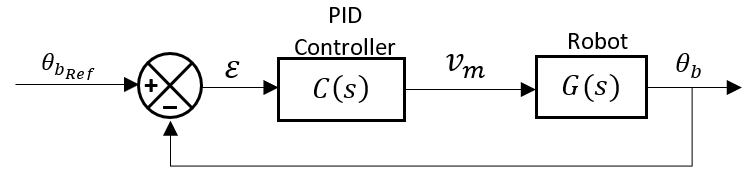
\includegraphics[width=\linewidth]{LabA/clContSysGs.png}
  \caption{Closed loop continuous system}
  \label{fig:fig1}
\end{figure}

With the following system and controller transfer functions:
\begin{equation*}
G(s)=\frac{Ks}{(s-p_1)(s-p_2)(s-p_3)}
\end{equation*}
\begin{equation*}
C(s)=K_p+K_i\frac{1}{s}+K_ds=\frac{K_ds^2+K_ps+K_i}{s}
\end{equation*}

Here is the closed-loop transfer funtion:
\begin{equation*}
H_{CL}(s)=\frac{C(s)G(s)}{1+C(s)G(s)}=\frac{K(K_ds^2+K_ps+K_i)}{(s-p_1)(s-p_2)(s-p_3)+K(K_ds^2+K_ps+K_i)}
\end{equation*}
Therefore the developped denominator of $H_{CL}$ is:
\begin{equation*}
P(s)=s^3+s^2(KK_d-p_1-p_2-p_3)+s(KK_p+p_1p_2+p_2p_3+p_1p_3)+KK_i-p_1p_2p_3
\end{equation*}

We already know that our plant has got 3 poles, one of which is unstable ($p_2>0$). Therefore, we will try to replace this pole with a stable one and end up with the following closed-loop denominator:
\begin{equation*}
P(s)=(s-p_1)(s-Q)(s-p_3)=s^3+s^2(-p_1-Q-p_3)+s(p_1Q+p_3Q+p_1p_3)-p_1p_3Q
\end{equation*}
With a purely real negative $Q$ we will have a stable system without oscillations. Then we can identify the terms between the polynom we have and the one we want to obtain the following equations system and therefore deduce the PID's parameters:
\begin{align*}
\begin{cases}
KK_d-p_1-p_2-p_3=-p_1-Q-p_3 \\
KK_p+p_1p_2+p_2p_3+p_1p_3=p_1p_3+p_1Q+p_3Q \\
KK_i-p_1p_2p_3=-p_1p_3Q
\end{cases}
\implies
\begin{cases}
K_d=\frac{p_2-Q}{K} \\
K_p=\frac{p_1Q+p_3Q-p_1p_2-p_2p_3}{K} \\
K_i=\frac{p_1p_2p_3-p_1p_3Q}{K}
\end{cases}
\end{align*}

We want the impulse response to asymptotically reach the null angle as this is our reference angle. The transient response is not important as the impulse input itself is not physically meaningful.\\

%/////4.3.2/////%
4.3.2 With $Q=-30$ we obtain the following PID parameters:
\begin{align*}
\begin{cases}
K_p=-193.31 \\
K_i=-1.1.10^3 s \\
K_d=-0.23 s
\end{cases}
\end{align*}

%/////4.3.3/////%
4.3.3 And this closed-loop transfer function:
\begin{equation*}
H_{CL}(s)=\frac{35.68s^4+3.029.10^4s^3+1.7.10^5s^2}{s^5+879s^4+3.023.10^4s^3+1.4.10^5s^2}
\approx \frac{1}{1+0.3s}
\end{equation*}
The first order system is obtained after approximating and canceling zeroes and poles using Matlab's \emph{minreal} tool. It helps us to predict the overall system's behaviour (it should be close to a regular first order system).\\
We keep the full system and obtain the following impulse response:
\begin{figure}[H]
  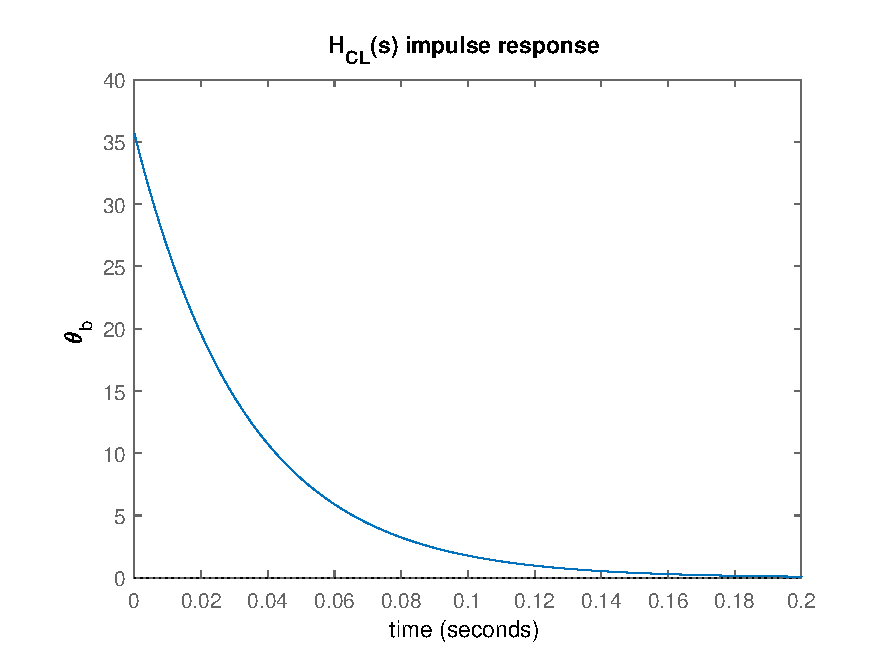
\includegraphics[width=\linewidth]{LabA/Task43_ImpulseResponse.pdf}
  \caption{$H_CL(s)$ impulse response}
  \label{fig:fig2}
\end{figure}
The system asymptotically reaches 0, this is what we want.

%/////////////////////////////////////////////////////////////%
%/////////////////////////TASK 4.4/////////////////////////%
%/////////////////////////////////////////////////////////////%
\subsection*{Reporting of Task 4.4}

%/////4.4.1/////%
4.4.1 We start with adding the disturbance $d$ to $Fx$:
\begin{equation*}
Fx+d=m_b \ddot x_b
\end{equation*}

The updated EOM in parametric form are: 
\begin{align*}
\begin{cases}
m_bl_b\ddot x_w + (I_b+m_b l_b^2)\ddot\theta_b =
m_bl_bg\theta_b-\frac{2K_t}{R_m}v_m+(\frac{2K_eK_t}{Rm}+b_f)(\frac{\dot x_w}{l_w}-\dot\theta_b)+d l_b\\
(\frac{I_w}{l_w}+l_wm_b+l_wm_w)\ddot x_w + m_bl_bl_w\ddot\theta_b =
\frac{2K_t}{R_m}v_m-(\frac{2K_eK_t}{Rm}+b_f)(\frac{\dot x_w}{l_w}-\dot\theta_b)+d l_w
\end{cases}
\end{align*}
													
%/////4.4.2/////%
4.4.2 We can now compute the new state space model:
\begin{equation*}
\begin{bmatrix}
	\dot x_w\\
     \ddot x_w\\
     \dot \theta_b\\
	\ddot \theta_b\\
	\end{bmatrix}
=
\begin{bmatrix}
0 & 1 & 0 & 0 \\
0 & -773.79 & -6.57 & 16.25 \\
0 & 0 & 0 & 1 \\
0 & 3313.24 & 63.07 & -69.58
\end{bmatrix}
\
\begin{bmatrix}
	x_w\\
	\dot x_w\\
	\theta_b\\
	\dot \theta_b
	\end{bmatrix}
+
\begin{bmatrix}
0 & 0 \\
36.6 & 1.88 \\
0 & 0\\
-156.71 & 1.08
\end{bmatrix}
\
\begin{bmatrix}
v_m \\
d
\end{bmatrix}
\end{equation*}

\begin{equation*}
\theta_b = 
\begin{bmatrix}
0 & 0 & 1 & 0\\
\end{bmatrix}
\
\begin{bmatrix}
	x_w\\
	\dot x_w\\
	\theta_b\\
	\dot \theta_b
	\end{bmatrix}
\end{equation*}


%/////////////////////////////////////////////////////////////%
%/////////////////////////TASK 4.5/////////////////////////%
%/////////////////////////////////////////////////////////////%
\subsection*{Reporting of Task 4.5}

%/////4.5.1/////%
4.5.1 Here is the simulink scheme we implemented with the new $A$, $B$, $C$ and $D$ matrices:
\begin{figure}[H]
  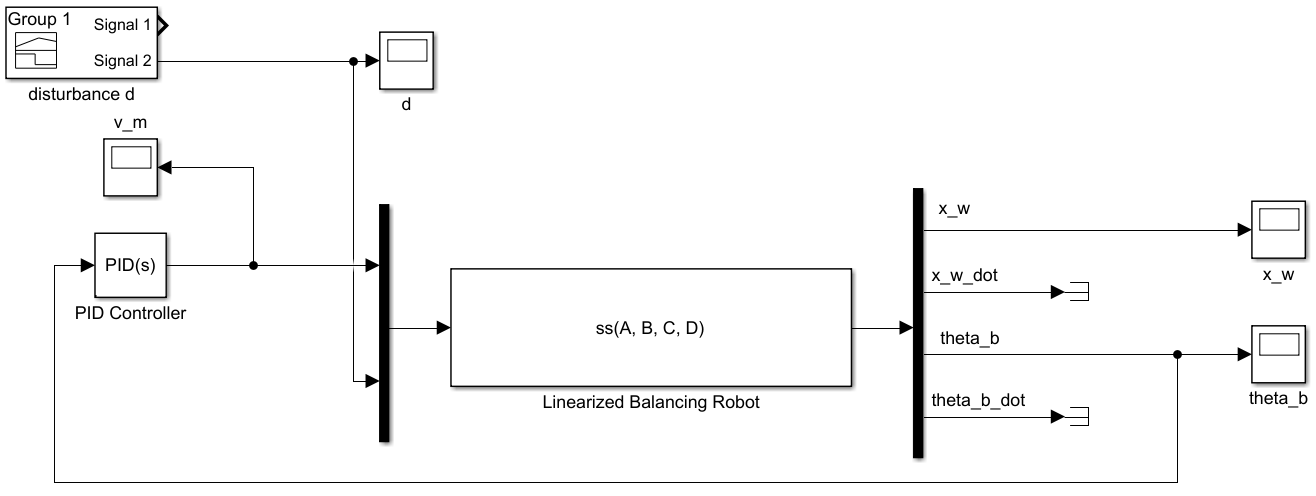
\includegraphics[width=\linewidth]{LabA/Task45_Simulink.png}
  \caption{Simulink model}
  \label{fig:fig3}
\end{figure}
The unused Signal 1 is a delayed disturbance, to ensure that the system is stable even before applying the $d$ force.
\newpage
%/////4.5.2/////%
4.5.2 Here are the results of the simulation:
\begin{figure}[H]
  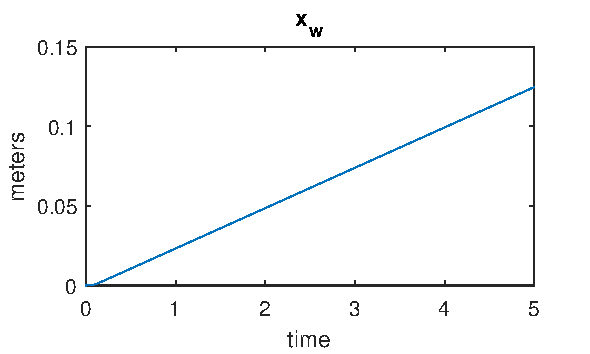
\includegraphics[width=\linewidth/2]{LabA/Task45_xw.pdf}
  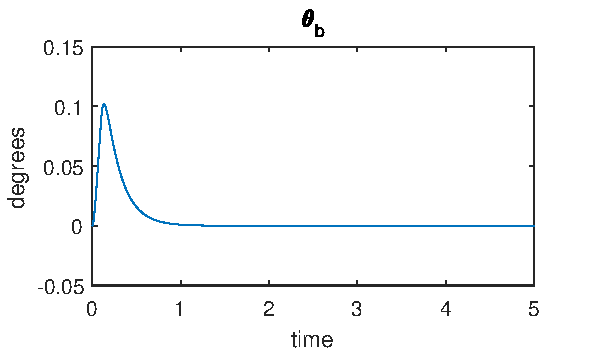
\includegraphics[width=\linewidth/2]{LabA/Task45_Thetaw.pdf}
  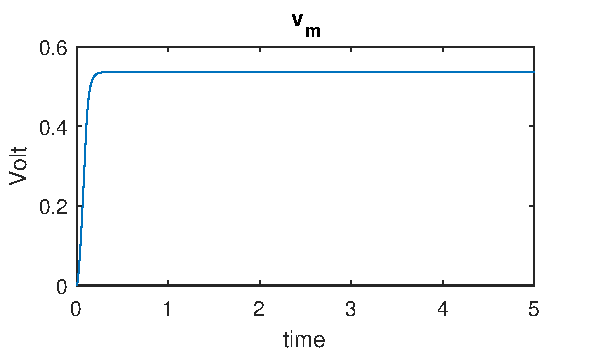
\includegraphics[width=\linewidth/2]{LabA/Task45_vw.pdf}
  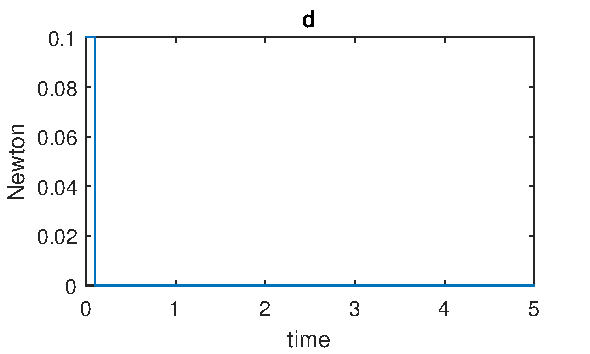
\includegraphics[width=\linewidth/2]{LabA/Task45_d.pdf}
  \caption{Simulation results}
  \label{fig:fig4}
\end{figure}
One can see that the robot moves forward to prevent itself from falling, but it keeps moving forward after (i.e. $x_w$ is always increasing, it is not stable). The angle $\theta_b$ is stabilized to $0$° despite the initial disturbance $d$. The command $v_m$ is stabilized at ~$0.5$ Volts. This is a realisitic value that could be provided by the battery.


%/////////////////////////////////////////////////////////////%
%/////////////////////////TASK 4.6/////////////////////////%
%/////////////////////////////////////////////////////////////%
\subsection*{Reporting of Task 4.6}
%/////4.6.1/////%
4.6.1 Using Matlab tools, we compute $H_{CL}(s)$'s bandwidth and find $\omega_{max}=30 rad.s^{-1}$.

%/////4.6.2/////%
4.6.2 Therefore, to comply with Nyquist-Shannon criterion, we must chose a sampling time $h$ as follow:
\begin{equation*}
\omega_{ech}>2\omega_{max}
\Leftrightarrow
h<\frac{2\pi}{2\omega_{max}}
\end{equation*}
To increase the margin we will take:
\begin{equation*}
h=\frac{2\pi}{5\omega_{max}}=42 ms
\end{equation*}
This value gives us more margin but should be high enough to be supported by the Arduino board.

%/////4.6.3/////%
4.6.3 We were not sure which bandwidth we should compute between $G(s)$ alone or $H_{CL}(s)$. Because some of us argued that we will sample only signal coming from outside $G(s)$ via the feedback loop, therefore we should comply to $G(s)$ bandwidth. Others said that the controller is part of the system, therefore it will produce frequencies that we should be able to sample correctly. Not knowing how to solve this issue, we decided to comply to the worst case in order to be sure that our sampling time will comply to both hypothesis. We had $\omega_{maxG(s)}=13.6 rad.s^{-1}$ and $\omega_{maxH_{CL}(s)}=30 rad.s^{-1}$. That's why we chose the closed-loop.

%/////4.6.4/////%
4.6.4 We can now discretize the controller using ZOH method. Here are the equivalences of $C(s)$'s proportionnal, integrative and derivative components between Laplace domain and Z domain:
\begin{align*}
\begin{cases}
P(s)=K_p(\Theta_{b_{Ref}}(s)-\Theta_b(s)) \\
I(s)=\frac{K_i}{s}(\Theta_{b_{Ref}}(s)-\Theta_b(s)) \\
D(s)=-K_ds\Theta_b(s)
\end{cases}
\Rightarrow
\begin{cases}
P(z)=K_p(\Theta_{b_{Ref}}(z)-\Theta_b(z)) \\
I(z)=\frac{K_ih}{z-1}(\Theta_{b_{Ref}}(z)-\Theta_b(z)) \\
D(z)=-\frac{K_d}{h}\frac{z-1}{z}\Theta_b(z)
\end{cases}
\end{align*}
Here, $\Theta_{b_{Ref}}$ is always the null angle.
Therefore, in discrete time domain we will implement this differential equation:
\begin{equation*}
v_m(k)=-K_p\theta_b(k) -K_i\sum\limits_{n = - \infty }^{k-1}{\theta_b(n)} - \frac{K_d}{h}(\theta_b(k)-\theta_b(k-1)
\end{equation*}


%/////////////////////////////////////////////////////////////%
%/////////////////////////TASK 4.7/////////////////////////%
%/////////////////////////////////////////////////////////////%
\subsection*{Reporting of Task 4.7}
%/////4.7.1/////%
4.7.1 We tried our \textbf{continuous controller} over the linearized and non-linearized simulators. In the non-linear system, the robot falls at $d=1.4N$.
Then we tried our \textbf{discrete controller}. In the non-linear system, the robot falls at $d=1.36N$.

%/////4.7.2/////%
4.7.2 Here are simulations of both controllers on each simulator (the disturbance is set just under the falling value):
\begin{figure}[H]
  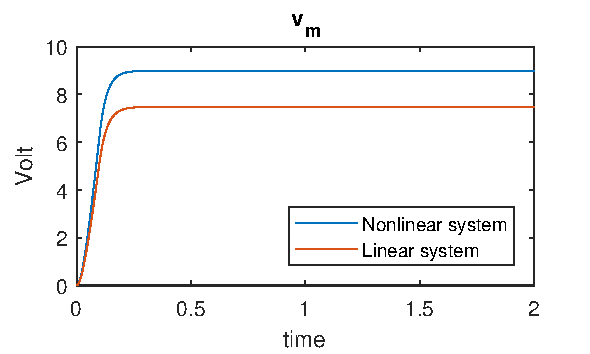
\includegraphics[width=\linewidth/2]{LabA/Task47_vmCont.pdf}
  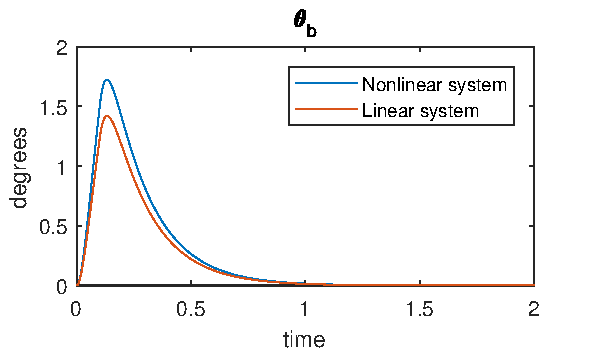
\includegraphics[width=\linewidth/2]{LabA/Task47_ThetawCont.pdf}
  \caption{Simulation with continuous time controller $C(s)$ and $d=1.395N$}
  \label{fig:fig5}
\end{figure}
\begin{figure}[H]
  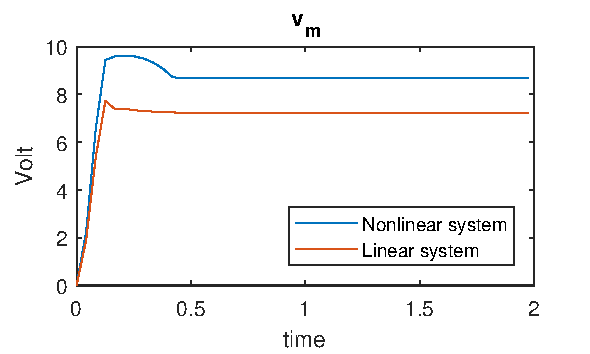
\includegraphics[width=\linewidth/2]{LabA/Task47_vmDisc.pdf}
  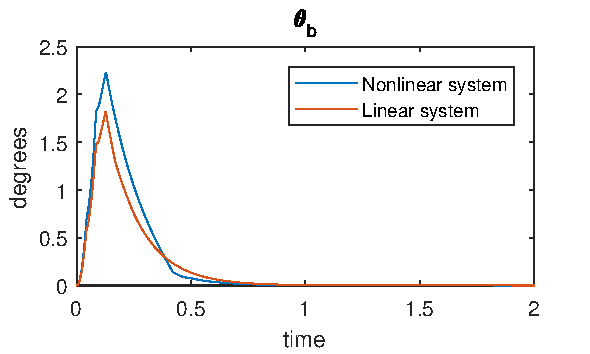
\includegraphics[width=\linewidth/2]{LabA/Task47_ThetawDisc.pdf}
  \caption{Simulation with discrete time controller $C(z)$ and $d=1.35N$}
  \label{fig:fig6}
\end{figure}

%/////4.7.3/////%
4.7.3 In both cases, we have $\theta_b^{lin} < \theta_b$. Therefore the controller is forced to provide a higher command to stabilize the nonlinear system, because of new forces that were not in the linear model. In reality, this may not work because we are exceeding the nominal value that batteries are able to provide (7.2V), i.e. the robot may fall with a smaller disturbance. Apart from this, one can see that with the discretized controller the responses are very similar to the full-continuous system. This is due to our sampling time that is quite short.

The worst sampling time we can take while staying in the Shannon-allowed range is $h=100 ms$. In that case, the system is already not stable anymore. The robot doesn't fall but ocillates around the null angle (marginal stability).  $h=70 ms$ is approximately the higher sampling time we can choose whithout having unstable system, more than that makes the robot oscillating after several seconds.

Then it is interesting to see that the extra mass can have the effect to slow down the robot. As we can see in figure \ref{fig:fig7}, the more mass we put and lower is the needed command voltage. Of, course there is a limit to this and for too heavy masses, the robot is not stable anymore (anyway in reality such masses can't be held by the robot).

\begin{figure}[H]
\begin{subfigure}[b]{0.5\linewidth}
  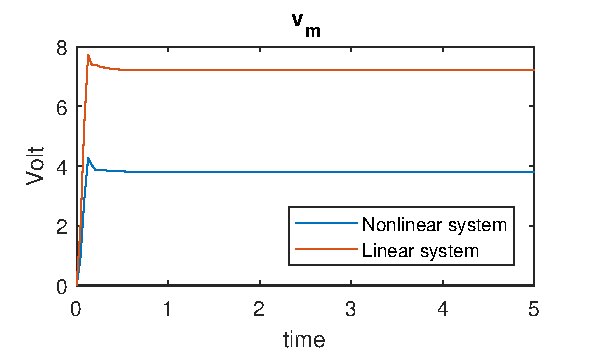
\includegraphics[width=\linewidth]{LabA/Task48_vmDiscXTraMass0kg500g.pdf}
  \caption{extra mass 500g}
\end{subfigure}
\begin{subfigure}[b]{0.5\linewidth}
  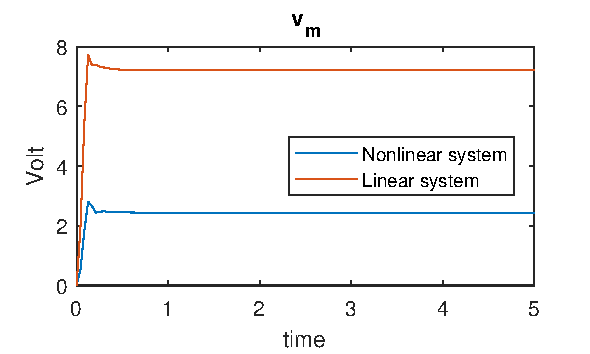
\includegraphics[width=\linewidth]{LabA/Task48_vmDiscXTraMass1kg.pdf}
    \caption{extra mass 1kg}
\end{subfigure}
\begin{subfigure}[b]{0.5\linewidth}
  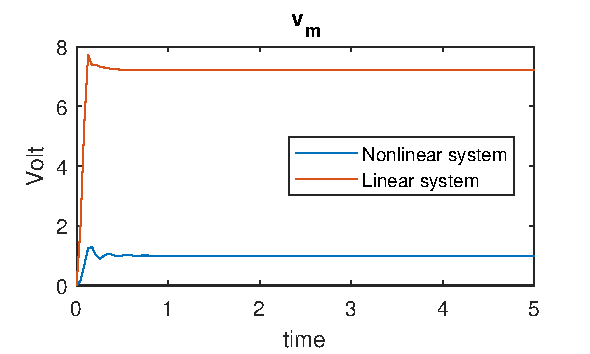
\includegraphics[width=\linewidth]{LabA/Task48_vmDiscXTraMass3kg.pdf}
    \caption{extra mass 3kg}
\end{subfigure}
\begin{subfigure}[b]{0.5\linewidth}
  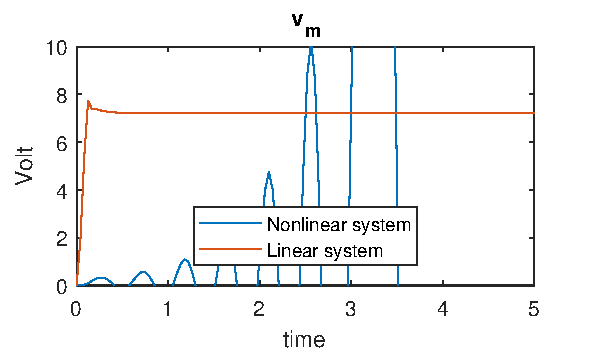
\includegraphics[width=\linewidth]{LabA/Task48_vmDiscXTraMass25kg.pdf}
    \caption{extra mass 25g}
\end{subfigure}
  \caption{Simulation with $C(z)$, $d=1.35N$ and extra masses}
  \label{fig:fig7}
\end{figure}

\subsection*{Lab A conclusion}
After establishing the state space representation of the system, we were able to design a continuous-time controller thanks to pole placement method. Then we simulated this controller (continuous and discretized) along with linear and nonlinear systems to test its robustness. During this lab we had lot of troubles to find the initial ss representation because we took a unconvenient $x$ vector. Then the other part that took us lot of time was the PID design with pole placement. We had several ideas but none of them worked (we tried root-locus method, poles cancellation and even the full-state feedback method...). Finally after re-thinking our solution and asking some hints to the teachers, we found a PID that stabilizes the system using a realistic command.

\end{document}
